\documentclass[12pt]{article}
\usepackage{ctex}
\usepackage{graphicx}
\usepackage{indentfirst}
\usepackage{amsmath}
\usepackage{amssymb}

\title{第三周作业报告}
\author{佐藤拓未 20300186002}
\date{}

\begin{document}
	\maketitle
	\begin{center}
	\textbf{第一问}
	\end{center}
	对于Hermite型插值多项式,要求节点函数值和一阶导数值,则有$N=2n-1$,证明其插值误差满足:$$f(x)-H_N(x)=\frac{f^{(N+1)}(\zeta)}{(N+1)!}\prod_{i=1}^n(x-x_i)^2$$
	\\
	\noindent \textbf{证明:}已知$H_N^{(j)}(x_i)=f^{(j)}(x_i)$,其中$0\le{j}\le{1}$,$1\le{i}\le{n}$\\
	记$r(x)=f(x)-H_N(x)$,$w_n(x)=\prod_{i=1}^n(x-x_i)^2$,若${x^'}\ne{x_j}$,则记$g(t)=r(t)-{\frac{r(x^')}{w_n(x^')}}w_n(t)$。\\
	那么$$g(x_i)=0;g({x^'})=0$$ $${g^'}(x_i)=0$$
	从而由罗尔定理:$\exists \{y_i\}_{i=1}^n\quad s.t.\quad {g'(y_i)}=0$,此时有$2n$个互异节点上有${g^'}$为0,则再由$2n-1$次罗尔定理可得$$g^{2n}(\zeta)=0$$
	由$H_N(x)$是$2n-1$次多项式,$w_n(x)$是$2n$次多项式,故有$$0=f^{2n}(\zeta)-(2n)!\frac{r({x^'})}{w_n({x^'})}$$
	从而

		\begin{align*}
			r({x^'})&=\frac{f^{2n}(\zeta)}{(2n)!}w_n({x^'})\\
			&=\frac{f^{(N+1)}(\zeta)}{(N+1)!}\prod_{i=1}^n({x^'}-x_i)^2
		\end{align*}
	\\
	\begin{center}
		\textbf{第二问}
	\end{center}
比较不同复化公式的误差行为,并考虑当$f(x)=\vert{x-\frac{1}{3}}\vert$时,在积分区间$[0,1]$用各种复化公式求积的精度\\
\\
\textbf{解:}利用MATLAB计算不同的复化积分公式,在不同个数的等距节点下,与$\int_{0}^1\vert{x-\frac{1}{3}}\vert dx=\frac{5}{18}$的误差$\beta=\vert{I-\int_{0}^1\vert{x-\frac{1}{3}}\vert dx}\vert$\\
考虑区间$[0,1]$上的分段个数$n=1,2,\dots,20$,并利用复化中点、梯形、Simpson以及$\frac{3}{8}$规则Simpson求积公式。\\
总体来说,复化Simpson求积公式关于$n$的收敛速度是最快,事实上,在$[0,1]$上的Simpson公式已经是精确值了;其次是复化$\frac{3}{8}$法则Simpson公式,其在$n=6$时的精度已经被控制在$1\times{10^{-3}}$以内;而复化中点公式与复化梯形公式的精度相当,前者与后者的精度分别在$n=11$与$n=13$时控制在$1\times{10^{-3}}$以内。\\
由于$\vert{x-\frac{1}{3}}\vert$在$[0,1]$上并不是全点可导:其在$x=\frac{1}{3}$处只存在左右导数,故导致复化梯形公式虽然$n=3$时的精度控制在$0.001$以内,但后续随着分段数$n$变大,其积分值产生了浮动,即虽然$\vert{x-\frac{1}{3}}\vert$是分段1次的,但原本具有1次代数精度的梯形求积公式不精确成立。\\
具体的图像如下:

\begin{figure}[h]
	\centering
	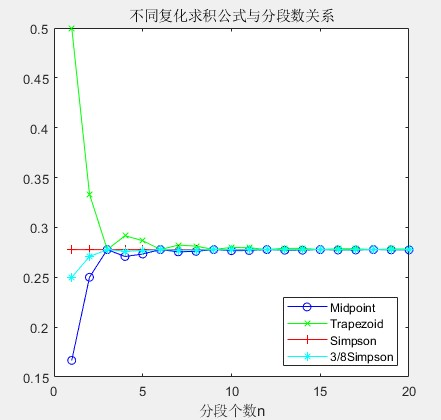
\includegraphics[width=1\textwidth]{1}
	\caption{横坐标对应了复化求积的分段个数;纵坐标对应了积分公式的积分值}
\end{figure}
\begin{figure}[h]
	\centering
	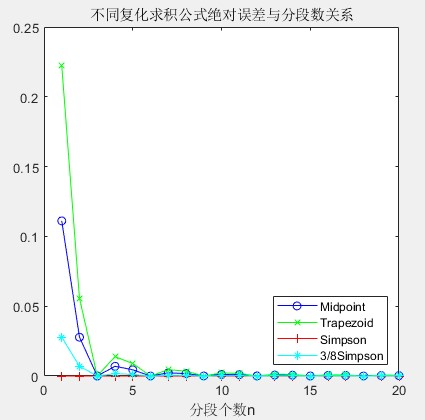
\includegraphics[width=1\textwidth]{2}
	\caption{横坐标对应了复化求积的分段个数;纵坐标对应了积分公式与精确值的绝对误差}
\end{figure}
\end{document}